\subsection{Rendering}
\paragraph{}
Rendering the scene into a perceivable image is one of the core jobs of the application.
Realizing effects that approximate both real movie footage and the wishes of the user is often hard, or even impossible.
The implementation is closely tied to the abilities requested from the tool, many effects such as lighting or arbitrary depth ordering requires low level trickery with the chosen framework.

In addition, the scene does not only have to be rendered once but often twice.
Binocular vision infers depth relationships from slight differences in images taken from two separate viewpoints.

Section \ref{FrameworkOpenGL} discusses the choice of drawing framework.
Section \ref{RendCamera} discusses how a 3D scene gets mapped into a 2D image.
Section \ref{RendStereo} discusses stereo rendering methods.
Section \ref{ImplContainer} discusses the implementation of other effects.
For a high level description of many features see section \ref{sceneRep} on scene representation and \ref{Cues} on the topic of depth cues.


\subsubsection{Camera\label{RendCamera}}

\begin{figure*}[hbt]
\begin{center}
\subfigure[Perspective Cameras]{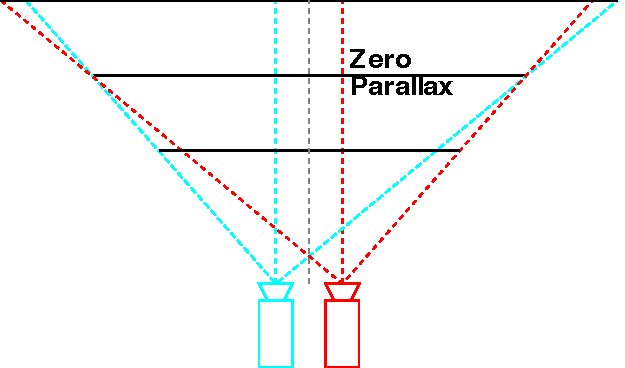
\includegraphics[scale=0.75]{media/camera-perspective.pdf}}
\subfigure[Parallel Cameras]{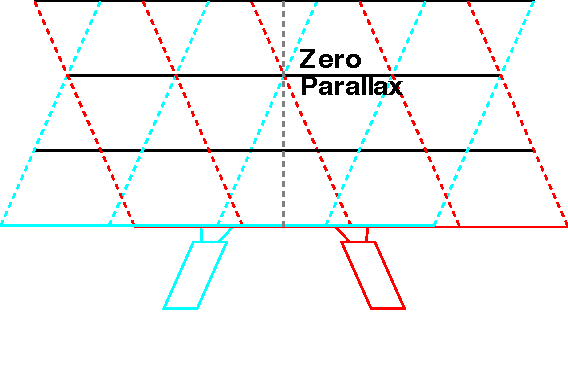
\includegraphics[scale=0.75]{media/camera-parallel.pdf}}
\caption{A diagram of the two main camera types}
\end{center}
\end{figure*}

\paragraph{}
\todo{Write about why it is important, in OpenGL}
\todo{Write about parallel perspective, parallel converged}

\subsubsection{Stereo\label{RendStereo}}
\paragraph{}
Ideally, the output of the program is either intended to be viewed without binocular vision, or a projector solution is used.
Then the scene is simply rendered twice into different windows or in split screen.
If the used graphic hardware supports it, \textit{OpenGL}'s QuadBuffering can be used to easily drive many types of stereoscopic viewing systems.

\paragraph{Anaglyph}
For a quick and easy preview on any screen, anaglyph is the simplest method.
Many different variations of anaglyph are used, the most popular of which are red-blue and red-green coding.
A simple implementation based could draw only the red channel of the image intended for the left eye, and the green and blue channel of the right eye.
Unfortunately this leads to rivalry when rendering scenes that contain objects that consist mostly of those colors.

The correct way is to mix all colors of one side into it's channel.
The loss of color contrast is made up with the better fuseability and the reduction in rivalry.

\todo{Write about rendering for stereoscopic vision, such as Anaglyph/SidebySide}

